\section{Обобщенная схема уязвимости системы аутентитфикации при различных
подходах к обеспечению безопасности}

Рассмотрев и классифицировав всевозможные виды уязвимостей различных узлов
открытых систем, а так же разновидности атак злоумышленников, построим
обобщенную схему уязвимости системы аутентификации пользователей в сети при
традиционном подходе, указав градации степени стойкости к вредоносным атакам
(Рис.~\ref{ris:2.1}).

\begin{figure}[h]
\center{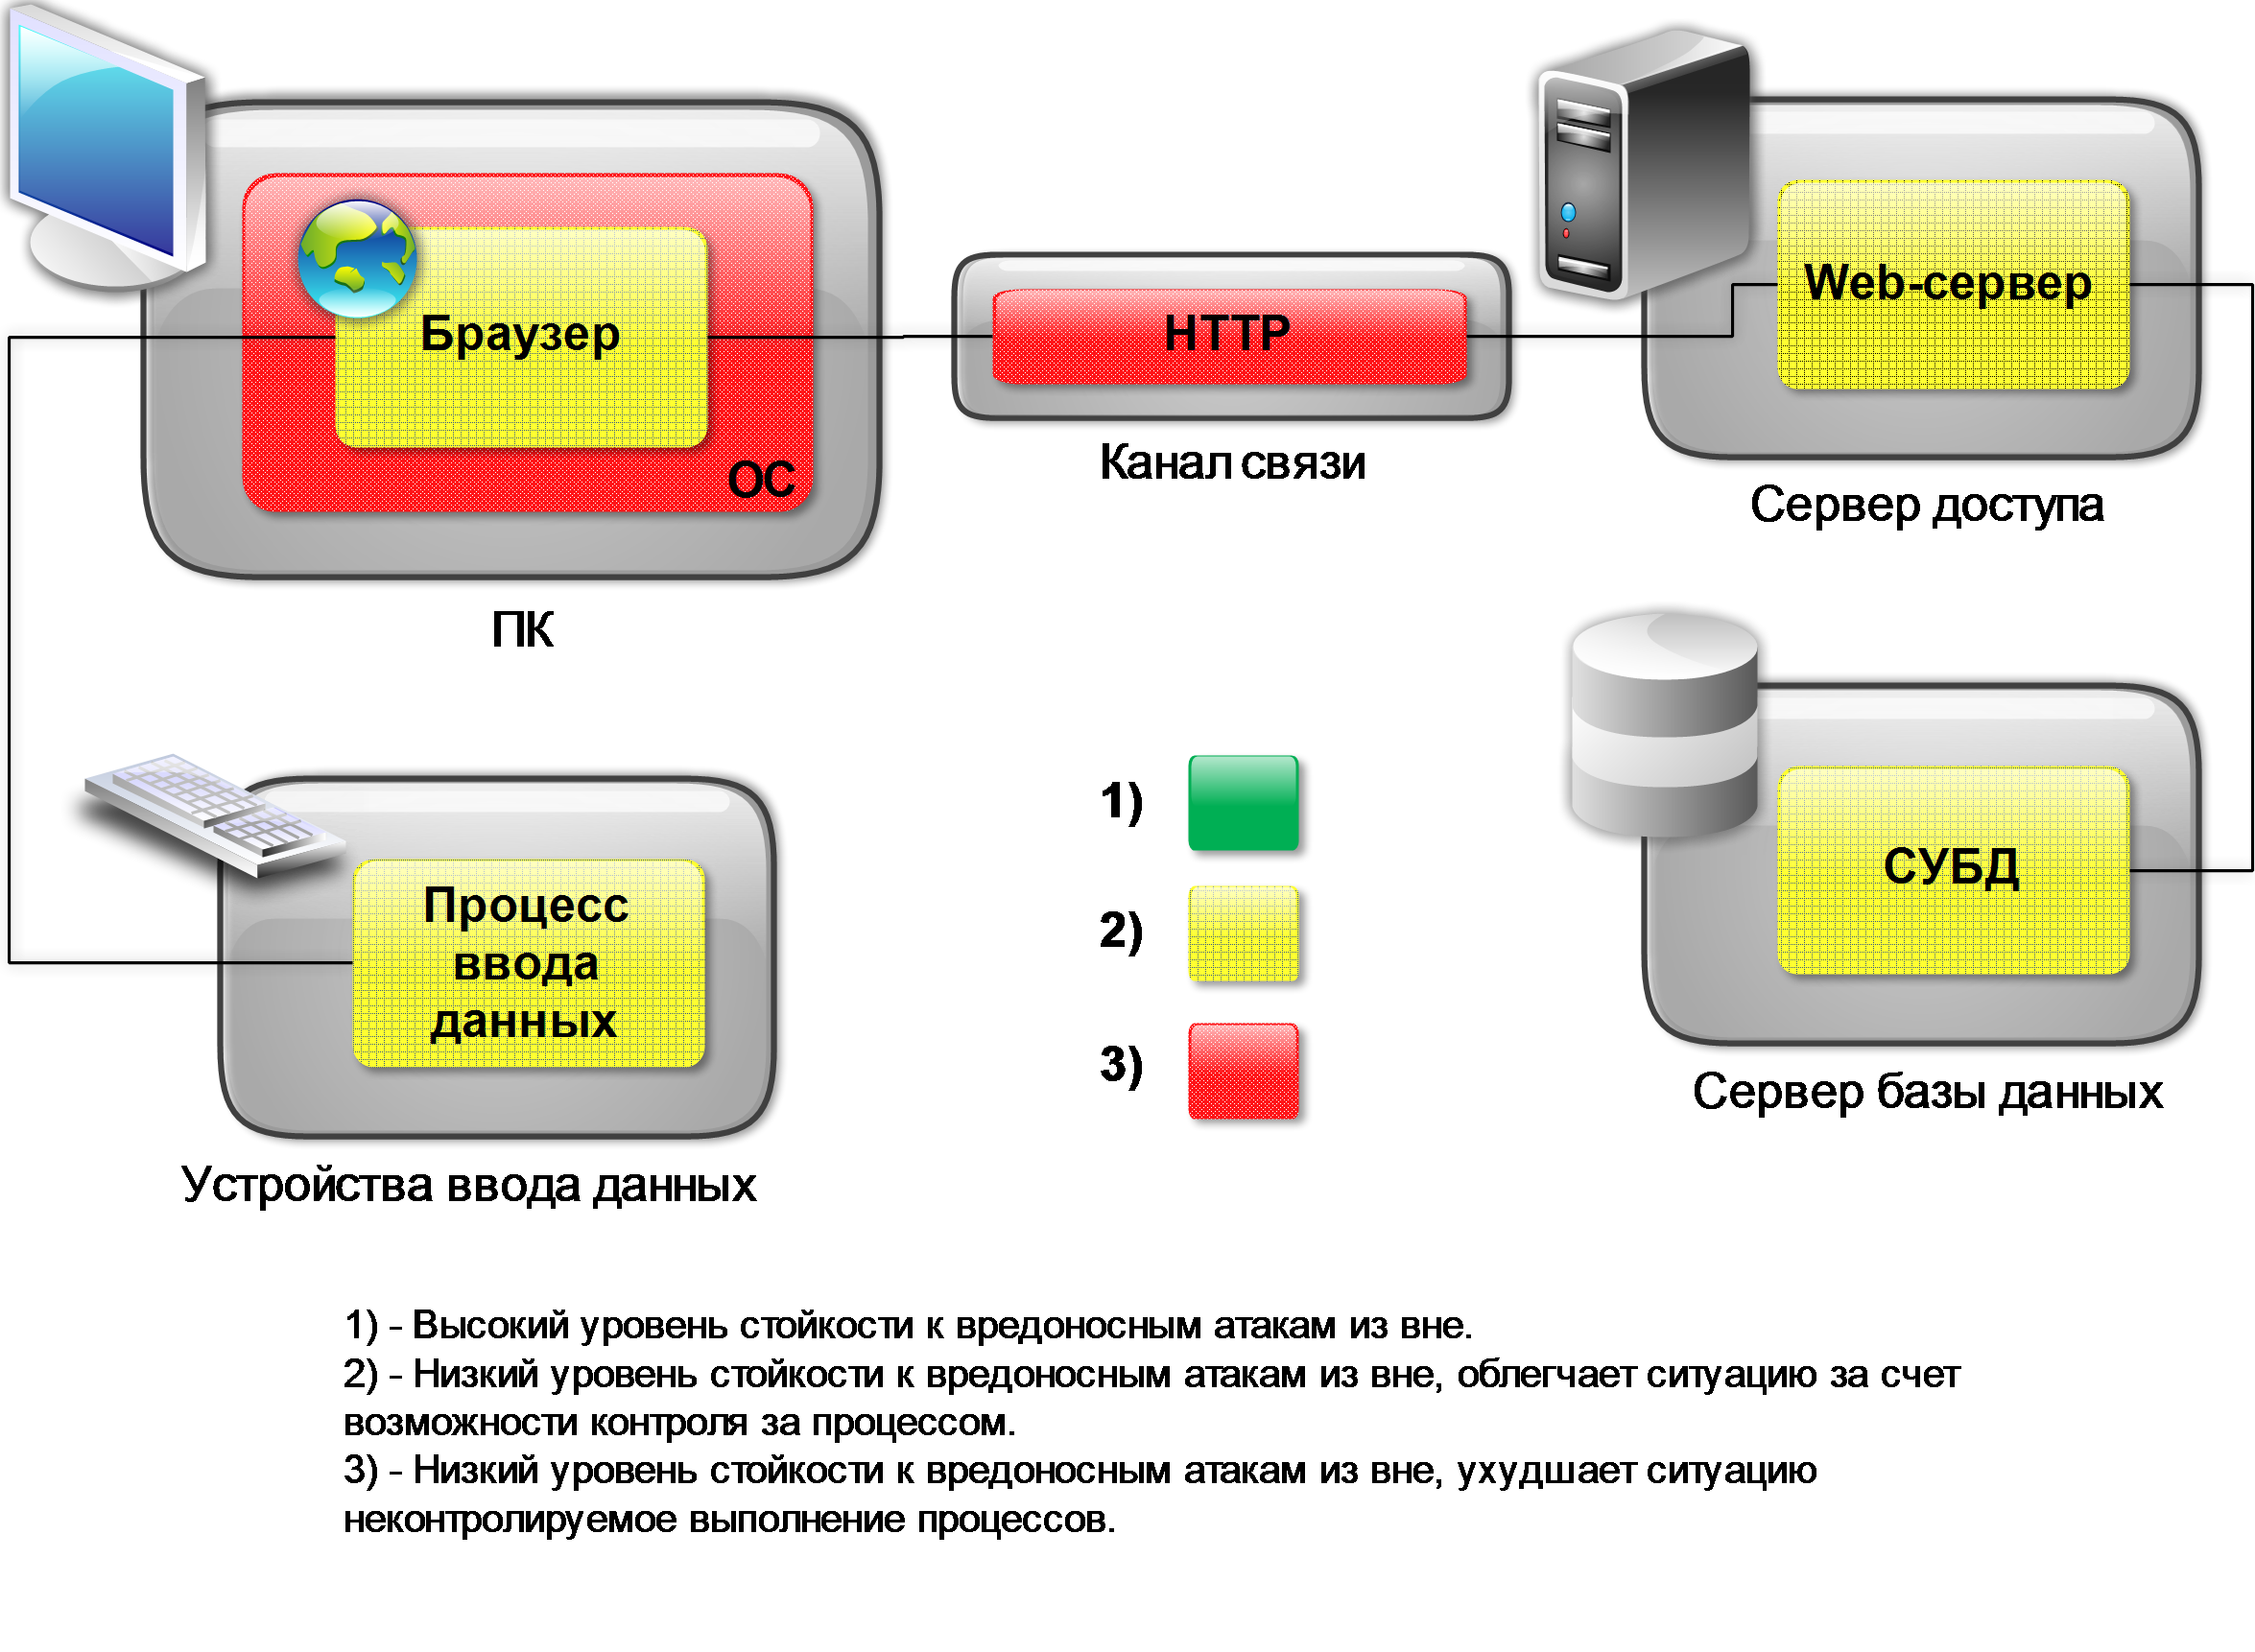
\includegraphics[width=1\linewidth]{2-1}}
\caption{Схема уязвимости узлов системы при традиционном подходе к
процессу аутентификации}
\label{ris:2.1}
\end{figure}

Детально рассмотрим уязвимости, которым подвержен каждый элемент системы в
отдельности.

\textit{Устройства ввода данных}, как правило, представляет собой клавиатуру. В
процессе аутентификации клавиатура может быть использована при вводе пароля. Данное
устройство включено в группу риска по следующим причинам:
\begin{itemize}
  \item данные (в частности пароль), вводимые с клавиатуры, могут быть
  доступными третьему лицу в результате банального слежения за процессом ввода;
  \item в результате целенаправленных действий злоумышленника клавиатура может
  быть сопряжена со специальным прослушивающим устройством, которое фиксирует
  все вводимые данные.
\end{itemize}

\textit{Персональный компьютер} входить в группу повышенной опасности из за
уязъвимостей операционных систем. В частности, угрозы могут исходить из
хаккерских атак, а так же от различных вредоносных программ, целенаправленно
собирающих секретную информацию. Ситуация осложняется из-за
неконтролируемого выполнения процессов, что не дает возможности определить
источник угрозы на ранних этапах.

\textit{Канал связи} является наиболее уязвимым местом любой системы, так как
информация передается абсолютно открытым образом, где практически каждый может
получить к ней доступ.

\textit{Серверная часть системы} так же включена в группу риска, не смотря на
высокие возможности обеспечения безопасности. Любая атака со стороны
злоумышленников может привести к полному отказу в работе системы и необратимым
последствиям.

Применение нового подхода к процессу аутентификации пользователей в сети с
использованием портативного цифрового ключа доступа снижает уровень уязвимости в
отдельных компонентах системы, особенно это касается критических участков. Это
можно проследить на рисунке~\ref{ris:2.2}).

 \begin{figure}[h]
\center{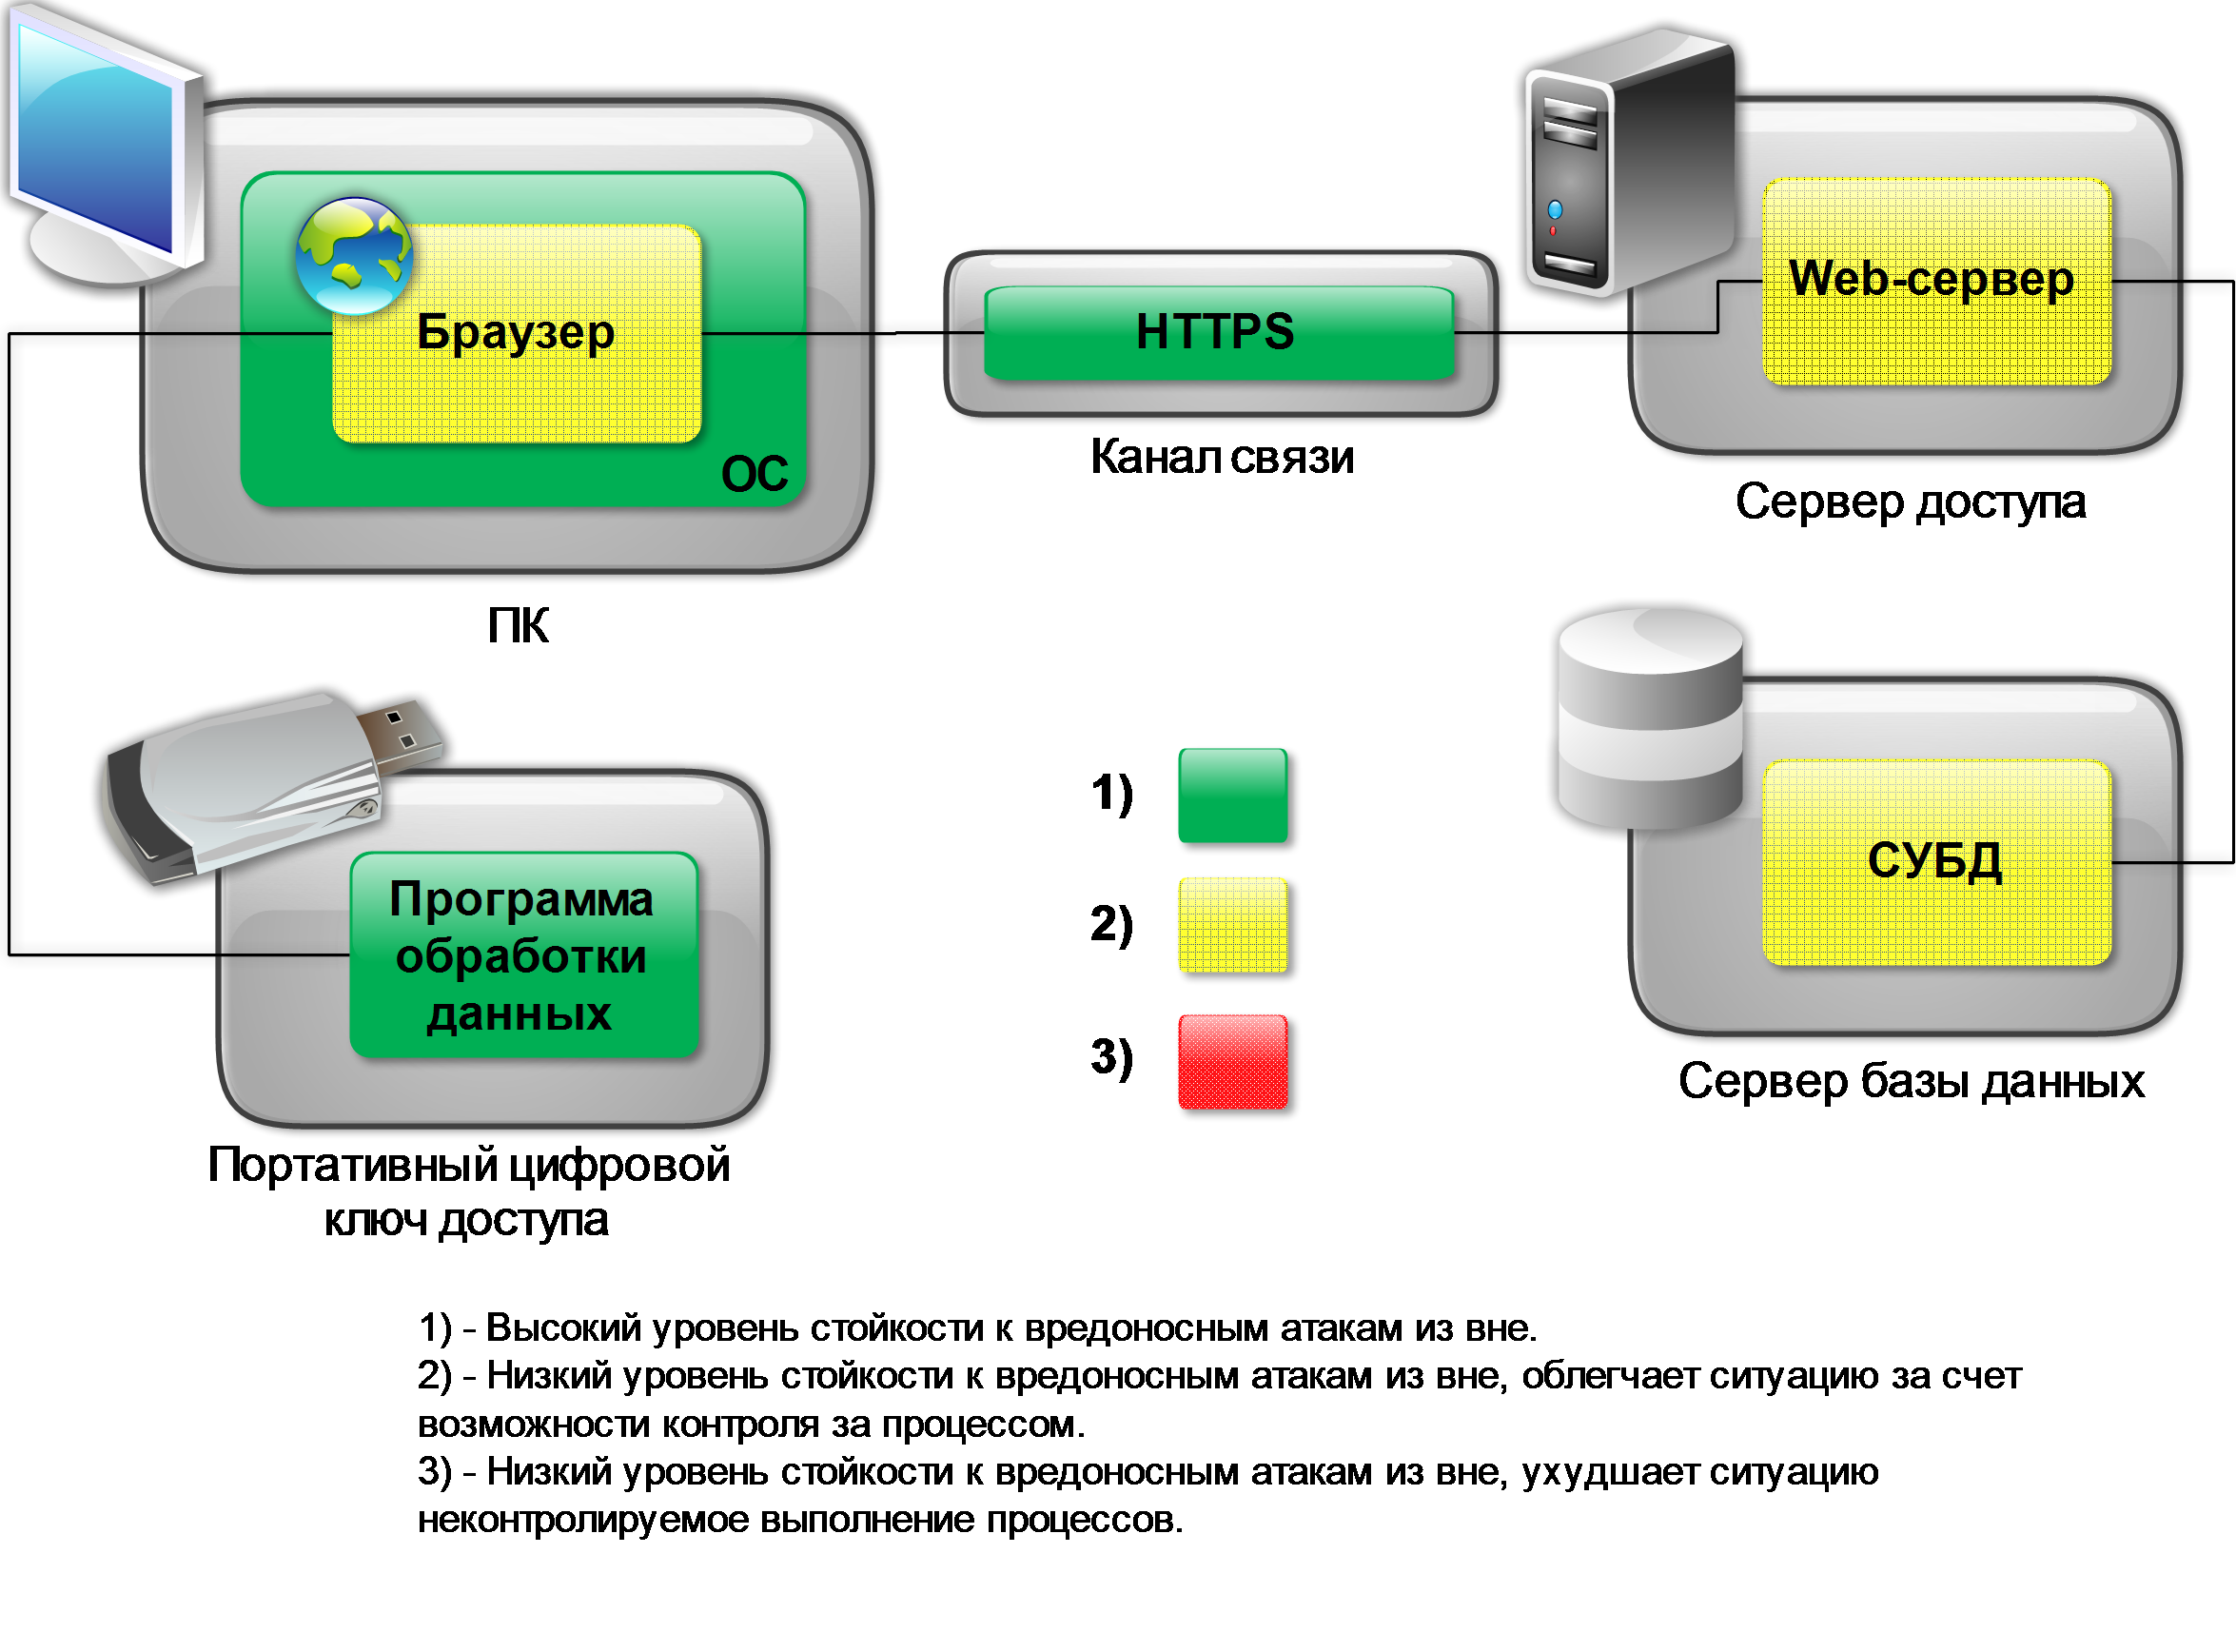
\includegraphics[width=1\linewidth]{2-2}}
\caption{Схема уязвимости узлов системы при новом подходе к процессу аутентификации}
\label{ris:2.2} 
\end{figure}


Выявленные улучшения достигаются с помощью:
\begin{itemize}
  \item Применяемых алгоритмов шифрования данных;
  \item Применения новой технологии хранения ключей и обработки алгоритмов
шифрования.
\end{itemize}

Применяемые алгоритмы шифрования обеспечивают безопасность передаваемых данных
при условии полной секретности ключей. 
  
Алгоритмы шифрования можно разделить на две категории:
\begin{itemize}
  \item алгоритмы симметричного шифрования;
  \item алгоритмы асимметричного шифрования.
\end{itemize}
	
В алгоритмах \textit{симметричного шифрования} для расшифрования обычно
используется тот же самый ключ, что и для зашифрования, или ключ, связанный с ним каким-либо
простым соотношением. Последнее встречается существенно реже, особенно в
современных алгоритмах шифрования. Такой ключ (общий для зашифрования и
расшифрования) обычно называется просто ключом шифрования.
Одним из наиболее распространенных алгоритмов данного вида является 
\textbf{DES} -- федеральный стандарт шифрования США в 1977-2001 годах,
разработанный группой под руководством доктора У. Тачмена. Архитектурой данного
алгоритма является классическая сбалансированная сеть Файстеля с начальной и
конечной битовыми перестановками общего вида. Длина ключа данного алгоритма
составляет 56 бит.

В \textit{асимметричном шифровании} ключ зашифрования $k_{1}$ легко вычисляется
из ключа $k_{2}$ таким образом, что обратное вычисление невозможно. Например, соотношение
ключей может быть таким:
\begin{equation}
k_{1} = a^{k_{2}} \ mod \ p ,
\end{equation}

где $a$ и $p$ -- параметры алгоритма шифрования, имеющие достаточно большую
размерность.

Яркими примерами данного вида шифрования являются алгоритмы \textbf{RSA} и
\textbf{ElGamal}.
Алгоритм RSA - Защищен патентом США N 4405829. Разработан в 1977 году в
Массачусетском технологическом институте (США). Получил название по первым
буквам фамилий авторов (Rivest, Shamir, Adleman). Криптостойкость основана на
вычислительной сложности задачи разложения большого числа на простые множители.
Алгоритм ElGamal разработан в 1985 году. Назван по фамилии автора - Эль-Гамаль.
Используется в стандарте США на цифровую подпись DSS (Digital Signature
Standard). Криптостойкость основана на вычислительной сложности задачи
логарифмирования целых чисел в конечных полях.~\cite{elgamal}

Еще одной разнавидностью асимметричных алгоритмов шифрования является
\textit{алгоритм электронно-цифровой подписи} (ЭЦП). Электронная подпись (ЭП) —
информация в электронной форме, которая присоединена к другой информации в электронной форме
(подписываемой информации) или иным образом связана с такой информацией и
которая используется для определения лица, подписывающего информацию.~\cite{FZ_63}
По своему существу электронная подпись представляет собой реквизит электронного
документа, позволяющий установить отсутствие искажения информации в электронном
документе с момента формирования ЭП и проверить принадлежность подписи владельцу
сертификата ключа ЭП. Значение реквизита получается в результате
криптографического преобразования информации с использованием закрытого ключа
ЭП.

Все существующие алгоритмы ЭЦП построены по единому принципу.
Разница заключается лишь в математической реализации отдельно взятого алгоритма.
Это связано с тем, что каждый новый алгоритм получает улучшения, по двум
основным направлениям:
повышение криптостойкости и снижение временных затрат и вычислительных ресурсов,
при этом схема генерации и верификации шифра остаётся неизменной.

Для уяснения сущности алгоритма рассмотрим математические принципы, на которых
они базируются. Все математические операции можно разделить на две части:
вычисление дайджеста подписываемого документа и сам алгоритм вычисления и
проверки шифра.
\begin{enumerate}
  \item Хеширование применяется для сравнения данных: если у двух массивов
  хеш-коды разные, массивы гарантированно различаются; если одинаковые --
  массивы, скорее всего, одинаковы. В общем случае однозначного соответствия
  между исходными данными и хеш-кодом нет в силу того, что количество значений
  хеш-функций меньше, чем вариантов входного массива; существует множество
  массивов, дающих одинаковые хеш-коды -- так называемые коллизии. Вероятность
  возникновения коллизий играет немаловажную роль в оценке качества хеш-функций.
Среди множества существующих хеш-функций принято выделять криптографически
стойкие, применяемые в криптографии. Для того, чтобы хеш-функция $H$ считалась
криптографически стойкой, она должна удовлетворять трем основным требованиям, на
которых основано большинство применений хеш-функций в криптографии:
	\begin{itemize}
	  \item Необратимость: для заданного значения хеш-функции m должно быть
	  вычислительно неосуществимо найти блок данных $X$, для которого $H(X) = m$;
	  \item Стойкость к коллизиям первого рода: для заданного сообщения $M$ должно
	  быть вычислительно неосуществимо подобрать другое сообщение $N$, для которого
	  $H(N) = H(M)$;
	  \item Стойкость к коллизиям второго рода: должно быть вычислительно
	  неосуществимо подобрать пару сообщений (М, М'), имеющих одинаковый хеш.
	\end{itemize}
	
Данные требования не являются независимыми:
  \begin{itemize}
    \item Обратимая функция нестойка к коллизиям первого и второго рода;
	\item Функция, нестойкая к коллизиям первого рода, нестойка к коллизиям второго
	рода; обратное неверно.
  \end{itemize}
	
Следует отметить, что не доказано существование необратимых хеш-функций, для
которых вычисление какого-либо прообраза заданного значения хеш-функции
теоретически невозможно. Обычно нахождение обратного значения является лишь
вычислительно сложной задачей.
Для криптографических хеш-функций также важно, чтобы при малейшем изменении
аргумента значение функции сильно изменялось (лавинный эффект). В частности,
значение хеша не должно давать утечки информации даже об отдельных битах
аргумента.~\cite{barichev}
  \item В источниках~\cite{GOST_P341094} и~\cite{ECP} описание алгоритма
  вычисления и проверки ЭЦП сформулированно следующим образом.
Пусть $x$ и $y$ это закрытый и открытый ключ соответственно. Такая пара является
единственной. Существует функция $y=p(x)$, которая связывает $x$ и $y$ и,
благодаря которой функции вычисления и проверки подписи становятся взаимообратными. Так же
существует группа параметров $Q$, которая является открытой, и не должна
меняться в пределах подписания и проверки одного документа. Пусть М -- текст
сообщения или документа, которые необходимо подписать с помощью электронной
подписи. Функция $h(M)$ вычисляет хеш сообщения. Пусть существует функция $t(x,
h(M), Q, k)$, где $k$ -- случайное число, генерируемое каждый раз, при
вычислении электронной подписи документа, тогда $r = t(x, h(M), Q, k)$ -- шифр,
существующая в открытом виде, доступная всем, а в первую очередь получателю.
Получателю известно само сообщение $M$, параметры алгоритма $Q$ и открытый ключ
отправителя $y$, а так же электронно-цифровая подпись к текущему документу,
которую сгенерировал отправитель,  назовём её $r'$, и, которая должна совпадать
с r, но возможно подверглась изменениям в результате действий злоумышленника.
Функция $v=t'(y, H(M), Q)$ вычисляет аналогичный шифр, но на данном этапе это
происходит уже с помощью открытого ключа. Таким образом, при равенстве $r'$ и
$v$ можно сделать вывод о том, что подпись и сам документ признается подлинным.
Существует важное ограничение, накладываемое на параметры $Q$. В силу того, что
в алгоритмах используются операция $mod$ (остаток от деления), не имеющая
обратной, тем самым обозначая логику защиты алгоритма, параметры $Q$ должны быть простые
числа. Кроме того, данные параметры должны быть «длинными» числами, причём, чем
«длиннее» число, тем выше криптостойкость алгоритма. Ключи алгоритма $x$ и $y$
берутся на основе параметров $Q$.
  \end{enumerate}

\textit{Новая технология} подразумевает использование специализированного
аппаратного средства для хранения ключей и обработки алгоритмов шифрования.
Данное устройство позволяет организовать безопасное хранение секретных ключей.
Программное средство, функционирующее на данном устройстве, предоставляет очень
узкий интерфейс обмена данными и малый набор команд, поэтому считать секретный
ключ с устройства не представляется возможным. Кроме того, для обеспечения
защиты ключа от несанкционированного копирования или кражи,  все алгоритмы
шифрования выполняются на данном устройстве. Таким образом, секретные ключи
имеют высочайшую степень защиты, что делает их абсолютно неуязвимыми на всех
этапах прохождения процедуры аутентификации пользователя в сети.

Кроме этого, помимо осуществления аутентификации пользователя в сети
корпоративных порталов, новая методика имеет широкие возможности для создания
инструментов проверки подлинности документов, поскольку данные процессы
практически идентичны с точки зрения реализации.
